% ===================================================================
%  Αρχείο: 15270_tikz.tex (Fragment)
%  Αυτόματη μετατροπή μέσω doc2latex.py & TikZ conversion
% ===================================================================

ΘΕΜΑ 2

Δίνεται η συνάρτηση $f(x) = \log_{\frac{1}{4}}(x)$.

\begin{alist}
\item Να βρείτε το πεδίο ορισμού της $f$. \monades{5}

\item Στο παρακάτω σχήμα δίνεται η γραφική παράσταση της $f$. 
\begin{rlist}
\item Να βρείτε, αν υπάρχουν, τα σημεία τομής της με τους άξονες. \monades{6}
\item Να βρείτε το σύνολο τιμών της $f$ και το διάστημα στο οποίο είναι γνησίως φθίνουσα. \monades{6}
\end{rlist}

\begin{center}
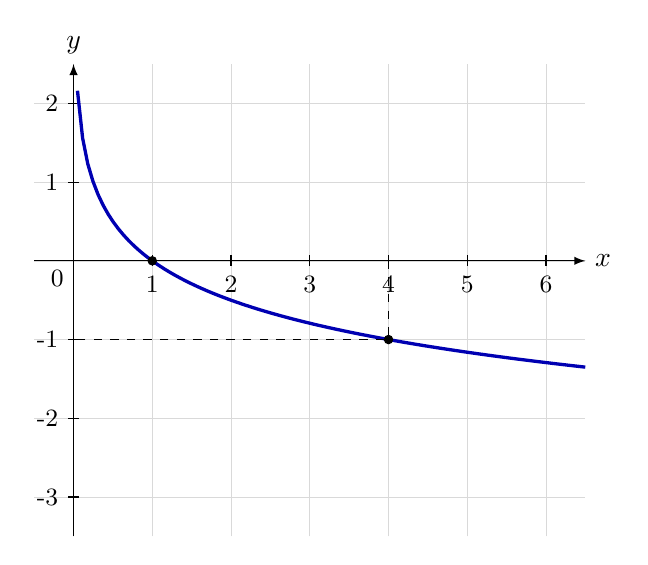
\begin{tikzpicture}[scale=1, >=latex]
    \draw[very thin, color=gray!30] (-0.5,-3.5) grid (6.5,2.5);
    \draw[->] (-0.5,0) -- (6.5,0) node[right] {$x$};
    \draw[->] (0,-3.5) -- (0,2.5) node[above] {$y$};
    
    \foreach \x in {1,2,3,4,5,6}
        \draw (\x,2pt) -- (\x,-2pt) node[below, font=\small] {\x};
    \foreach \y in {-3,-2,-1,1,2}
        \draw (2pt,\y) -- (-2pt,\y) node[left, font=\small] {\y};
    \node[below left, font=\small] at (0,0) {$0$};
    
    % f(x) = log_1/4 (x) = - ln(x) / ln(4)
    \draw[very thick, color=blue!70!black, samples=100, domain=0.05:6.5] plot (\x, {-ln(\x) / ln(4)});
    
    % Root (1,0)
    \filldraw (1,0) circle (1.5pt);
    % Point (4,-1)
    \draw[dashed] (4,0) -- (4,-1) -- (0,-1);
    \filldraw (4,-1) circle (1.5pt);
\end{tikzpicture}
\end{center}

\item Να αιτιολογήσετε το είδος μονοτονίας της. \monades{8}
\end{alist}
